\section{Hipster: Implementation and Use}
\label{sec:hipster}

We now give a description of the implementation of Hipster, and show how it can be used both in theory exploration mode and in proof mode, to find lemmas relevant for a particular proof attempt. An overview of Hipster is shown in figure \ref{fig:hipster}. The source code and examples are available online\footnote{\url{https://github.com/moajohansson/IsaHipster}}.

\begin{figure}[htbp]
\begin{center}
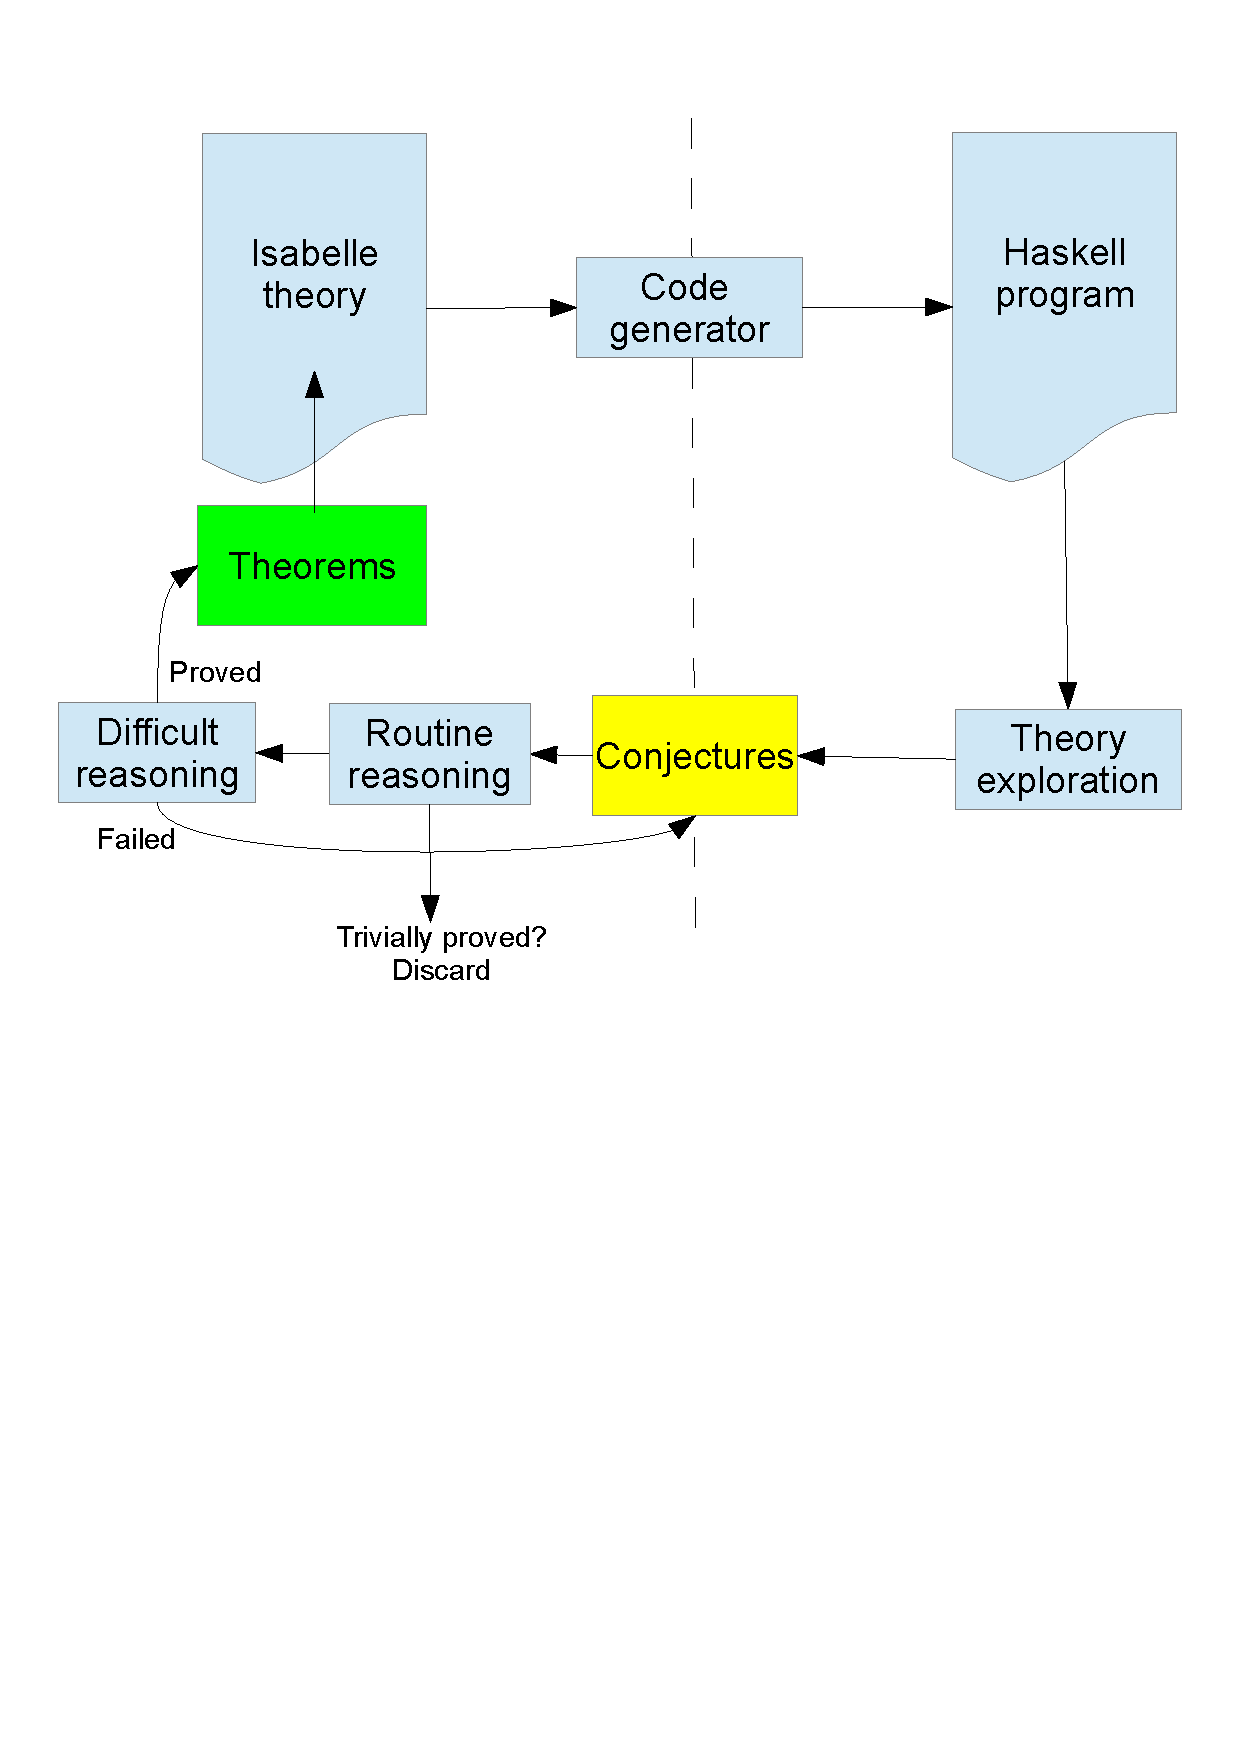
\includegraphics[scale=0.45]{hipster}

\caption{Overview of Hipster}
\label{fig:hipster}
\end{center}
\end{figure}

Starting from an Isabelle theory, Hipster calls Isabelle's code generator \cite{codegen} to translate the given functions into a Haskell program. In order to use the testing framework from QuickCheck, as described in the previous section, we must however also post-process the Haskell file, adding \emph{generators}, which are responsible for producing arbitrary values used for evaluation and testing. 
% Does anyone want to expand on exctly what we do?
%We use generators automatically deduced by the Feat package \cite{feat}. 
Another important issue that need to be addressed at this stage is the differences in semantics for partial functions in Isabelle and Haskell. In order to avoid HipSpec missing equations that hold in Isabelle, but not in Haskell, we had to modify the translation of partial functions. This is explained in more detail in section \ref{sec:partial}.

Once the Haskell program is in place, we run theory exploration and generate a set of equational conjectures, which HipSpec orders according to generality. More general equations are preferred, as we expect these to be more widely applicable as lemmas. In previous work on HipSpec, the system would at this stage apply induction on the conjectures and send them off to some external prover. Here, we instead import them back into Isabelle as we wish to produce checkable LCF-style proofs for our conjectures. 

The proof procedure in Hipster is parametrised by two tactics, one for easy or \emph{routine reasoning} and one for \emph{difficult reasoning}. In the examples below, we use Isabelle's simplifier followed by first-order reasoning by Metis \cite{metis} as routine reasoning, and a tactic performing structural induction followed by simplification and first-order reasoning as difficult reasoning. Metis is restricted to run for at most one second in both the routine and difficult tactic. If there are several possible variables to apply induction to, we may backtrack if the first choice fails. Both tactics have access to the theorems proved so far, and hence gets stronger as the proof procedure proceed through the list of conjectures. 

As there are rather many conjectures produced by theory exploration, we do not want to present them all to the user, but rather select the most interesting ones, which are difficult to prove. Those that follow only by routine reasoning are filtered out. 
Depending on the theory and application we can vary the tactics for routine- and difficult reasoning to suit our needs. If we want Hipster to produce fewer or more lemmas, we can choose a stronger or weaker tactic, allowing for flexibility.  

The order in which Hipster tries to prove things matter. As we mentioned, it will try more general conjectures first, with the hope that they will be useful to filter out many more specific routine results. Occasionally though, a proof will fail as a not yet proved lemma is required. In this case, the failed conjecture is added back into the list of open conjectures and retried later, provided that at least one new lemma has been proved in the meantime, to ensure progress and termination. Hipster terminates when it either runs out of open conjectures, or when it does not make any more progress. 

Below we give two typical use cases for Hipster. In both examples, Hipster has been instantiated with the  same routine- and difficult reasoning tactics, described above.

\subsection{Exploring a Theory of Binary Trees}
\label{sec:tree}
This example is about a theory of binary trees, with data stored at the leaves:
\begin{small}
\begin{verbatim}
datatype 'a Tree = 
    Leaf 'a 
  | Node "'a Tree" "'a Tree"
\end{verbatim}
\end{small}
Let's define some function over our trees: \texttt{mirror} swaps the left and right subtrees everywhere, and \texttt{tmap} applies a function to each element in the tree.
\begin{small}
\begin{verbatim}
fun mirror :: 'a Tree => 'a Tree
where
  mirror (Leaf x) = Leaf x
| mirror (Node l r) = Node (mirror r) (mirror l)

fun tmap :: ('a => 'b) => 'a Tree => 'b Tree
where
  tmap f (Leaf x) = Leaf (f x)
| tmap f (Node l r) = Node (tmap f l) (tmap f r) 
\end{verbatim} 
\end{small}
Now, let's call theory exploration to discover some properties about
these two functions. Hipster quickly finds and proves the two expected lemmas:
\begin{small}
\begin{verbatim}
lemma lemma_a [thy_expl]: "mirror (tmap x y) = tmap x (mirror y)"
by (tactic {* Hipster_Tacs.induct_simp_metis . . .*})

lemma lemma_aa [thy_expl]: "mirror (mirror x) = x"
by (tactic {* Hipster_Tacs.induct_simp_metis . . . *})
\end{verbatim}
\end{small}
The output produced by Hipster can be automatically pasted into the proof script by a mouseclick. Recall that Hipster discards all lemmas that can be proved by routine reasoning (here, without induction). The tactic \texttt{induct\_simp\_metis} appearing in the proof script output is the current instantiation of ``difficult reasoning''. Note that the lemmas discovered have been tagged with the attribute \texttt{thy\_expl}, which tells Hipster which lemmas it has discovered so far. If theory exploration is called several times, we can use these lemmas in proofs and avoid rediscovering the same things. The user can also inspect what theory exploration has found so far by executing the Isabelle command: \texttt{thm thy\_expl}.

Now, let's also define two functions extracting the leftmost and rightmost element of the tree:
\begin{small}
\begin{verbatim}
fun rightmost :: 'a Tree => 'a
where 
  rightmost (Leaf x) = x
|  rightmost (Node l r) = rightmost r

fun leftmost :: 'a Tree => 'a
where 
  leftmost (Leaf x) = x
|  leftmost (Node l r) = leftmost l
\end{verbatim}
\end{small}
Asking Hipster for lemmas about all the functions defined so far, it provides one additional lemma, namely:
\begin{small}
\begin{verbatim}
lemma lemma_ab [thy_expl]: "leftmost (mirror x2) = rightmost x2"
by (tactic {* Hipster_Tacs.induct_simp_metis . . . *})
\end{verbatim}
\end{small}
Finally, we define a function flattening trees to lists:
\begin{small}
\begin{verbatim}
fun flat_tree :: 'a Tree => 'a list
where
  flat_tree (Leaf x) = Cons x []
| flat_tree (Node l r) = (flat_tree l) @ (flat_tree r)
\end{verbatim}
\end{small}
We can now ask Hipster to explore the relationships between the functions on trees and the corresponding functions on lists, such as \texttt{rev}, \texttt{map} and \texttt{hd}. Hipster produce four new lemmas and one open conjecture:
\begin{small}
\begin{verbatim}
lemma lemma_ac [thy_expl]: "flat_tree (tmap x y) = map x (flat_tree y)"
by (tactic {* Hipster_Tacs.induct_simp_metis . . . *})

lemma lemma_ad [thy_expl]: "map x (rev xs) = rev (map x xs)"
by (tactic {* Hipster_Tacs.induct_simp_metis . . . *})

lemma lemma_ae [thy_expl]: "flat_tree (mirror x) = rev (flat_tree x)"
by (tactic {* Hipster_Tacs.induct_simp_metis . . . *})

lemma lemma_af [thy_expl]: "hd (xs @ xs) = hd xs"
by (tactic {* Hipster_Tacs.induct_simp_metis . . . *})

lemma unknown: "hd (flat_tree x) = leftmost x"
oops
\end{verbatim}
\end{small}
%flat_tree (tmap x y) = map x (flat_tree y)
%flat_tree (mirror x) = rev (flat_tree x)
%map x (rev xs) = rev (map x xs)
%hd (xs @ xs) = hd xs
Lemmas \texttt{ad} and \texttt{af} are perhaps not of much interest, as they only relate functions on lists. In fact, lemma \texttt{ad} is already in Isabelle's list library, but is not labelled as a simplification rule, why Hipster rediscovers it. Lemma \texttt{af} is a specialisation of a conditional library-lemma, with the side-condition that the first list is non-empty. Hipster can however not discover conditional lemmas, why the specialised version is produced instead. In addition to the four lemmas which have been proved, Hipster also outputs one interesting conjecture (labelled \texttt{unknown}) which it fails to prove. To prove this conjecture, we need a lemma stating that, as the trees store data at the leaves, \texttt{flat\_tree} will always produce a non-empty list:\\
 \texttt{flat\_tree t $\neq$ []}. As this is not an equation, it is
 not discovered by Hipster\footnote{If we also gave Hipster the
   constant $False$ as an input, it would discover the equation
  \texttt{(flat\_tree t = []) = False}, at the cost of increasing
  the size of the search space.}.
 
This example shows that Hipster indeed can find most of the basic lemmas we would expect in a new theory. The user has to provide the constants Hipster should explore, and the rest is fully automatic, thus speeding up theory development.  Theory exploration in this example takes just a few seconds, no longer that it takes to run tools like Sledgehammer. Even if Hipster fail to prove some properties, they may still be interesting, and the user can choose to prove them interactively.

\subsubsection*{Exploring with different tactics.}
To illustrate the effects of choosing a slightly different tactic for routine and difficult reasoning, we also experimented with an instantiation using only Isabelle's simplifier as routine reasoning and induction followed by simplification as difficult reasoning. The advantage of this instantiation is that the simplifier generally is faster than Metis, but less powerful. However, for this theory, it turns out that the simplifier is sufficient to prove the same lemmas as above. Hipster also suggests one extra lemma, namely \texttt{rightmost (mirror x) = leftmost x}, which is the dual to lemma \texttt{ab} above. When we used Metis, this lemma could be proved without induction, by routine reasoning, and was thus discarded. Using only the simplifier, difficult reasoning and induction is required to find a proof, and the lemma is therefore presented to the user. 

\subsection{Proving Correctness of a Small Compiler}
\label{sec:comp-ex}
The following example is about a compiler to a stack machine for a toy
language with generic types of expressions\footnote{This example is a slight variation of that in \S3.3 in the Isabelle tutorial \cite{isabelle}. }. We show how theory exploration can be used to unblock a proof on which automated tactics otherwise fail due to a missing lemma.

Expressions in the language are built from constants (\texttt{Cex}), values (\texttt{Vex}) and binary operators (\texttt{Bex}): 
\begin{small}
\begin{verbatim}
type_synonym 'c binop = 'c => 'c => 'c

datatype ('c, 'v) expr =
  Cex 'c |
  Vex 'v |
  Bex "'c binop" "('c,'v) expr" "('c,'v) expr"
\end{verbatim}
\end{small}
The types of variables and values are not fixed, but given by type parameters \texttt{'c} and \texttt{'v}.
To evaluate an expression, we define a function \texttt{value}, parametrised by an environment mapping variables to values:
\begin{small}
\begin{verbatim}
fun value :: ('v => 'c) => ('c,'v) expr => 'c
where
    value env (Cex c) = c 
  | value env (Vex v) = env v
  | value env (Bex b e1 e2) = b (value env e1) (value env e2)
\end{verbatim}
\end{small}
A program for our stack machine consists of four instructions:
\begin{small}
\begin{verbatim}
datatype ('c, 'v) program =
  Done
  | Const 'c "('c, 'v) program"
  | Load 'v "('c, 'v) program"
  | Apply "'c binop" "('c, 'v) program"
\end{verbatim}
\end{small}
A program is either empty (\texttt{Done}), or consists of one of the instructions \texttt{Const}, \texttt{Load} or \texttt{Apply}, followed by the remaining program. We further define a function \texttt{sequence} for combining programs:
\begin{small}
\begin{verbatim}
fun sequence :: ('c, 'v) program => ('c, 'v) program => ('c, 'v) program
where
    sequence Done p = p
  | sequence (Const c p) p' = Const c (sequence p p')
  | sequence (Load v p) p' = Load v (sequence p p')
  | sequence (Apply b p) p' = Apply b (sequence p p') 
\end{verbatim}
\end{small}
Program execution is modelled by the function \texttt{exec}, which given a store for variables and a program, returns the values on the stack after execution.
\begin{small}
\begin{verbatim}
fun exec :: ('v => 'c) =>  ('c,'v) program => 'c list => 'c list
where
    exec env Done stack = stack
  | exec env (Const c p) stack = exec env p (c#stack)
  | exec env (Load v p) stack = exec env p ((env v)#stack)
  | exec env (Apply b p) stack =
     exec env p ((b (hd stack) (hd(tl stack)))#(tl(tl stack)))
\end{verbatim}
\end{small}
We finally define a function \texttt{compile}, which specifies how expressions are compiled into programs:
\begin{small}
\begin{verbatim}
fun compile :: ('c,'v) expr => ('c,'v) program
  where
    compile (Cex c) =  Const c Done
  | compile (Vex v) =  Load v Done
  | compile (Bex b e1 e2) =
     sequence (compile e2) (sequence (compile e1) (Apply b Done))"
\end{verbatim}
\end{small}
Now, we wish to prove correctness of the compiler, namely that executing a compiled expression indeed results in the value of that expression: 
\begin{verbatim}
theorem "exec getBinop env (compile e) [] = [value getBinop env e]"
\end{verbatim}
If we try to apply induction on \texttt{e}, Isabelle's simplifier solves the base-case but neither the simplifier or first-order reasoning by Sledgehammer succeeds in proving the step-case. At this stage, we can apply Hipster's theory exploration tactic. It will generate a set of conjectures, and interleave proving these with trying to prove the open sub-goal. Once Hipster succeeds in finding a set of lemmas which allow the open goal to be proved by routine reasoning, it presents the user with a list of lemmas it has proved, in this case:
\begin{small}
\begin{verbatim}
Try first proving lemmas:

lemma lemma_a: "sequence x Done = x"
by (tactic {* Hipster_Tacs.induct_simp_metis . . . *})

lemma lemma_aa: "exec x y (sequence z x1) xs = exec x y x1 (exec x y z xs)"
by (tactic {* Hipster_Tacs.induct_simp_metis . . . *})

lemma lemma_ab: "exec x y (compile z) xs = value x y z # xs"
by (tactic {* Hipster_Tacs.induct_simp_metis . . . *})
\end{verbatim}
\end{small}
Pasting these into our proof script we can try Sledgehammer on our theorem again. This time, it succeeds and suggests the one line proof:% \texttt{by (metis lemma\_ab)}.
\begin{verbatim}
theorem "exec getBinop env (compile e) [] = [value getBinop env e]"
by (metis lemma_ab)
\end{verbatim}
Our theorem is a trivial instance of \verb|lemma_ab|, which in turn
depends on \verb|lemma_aa|. Hipster finds and proves both lemmas.
